% This file was created by matlab2tikz.
%
\definecolor{mycolor1}{rgb}{0.00000,0.44700,0.74100}%
%
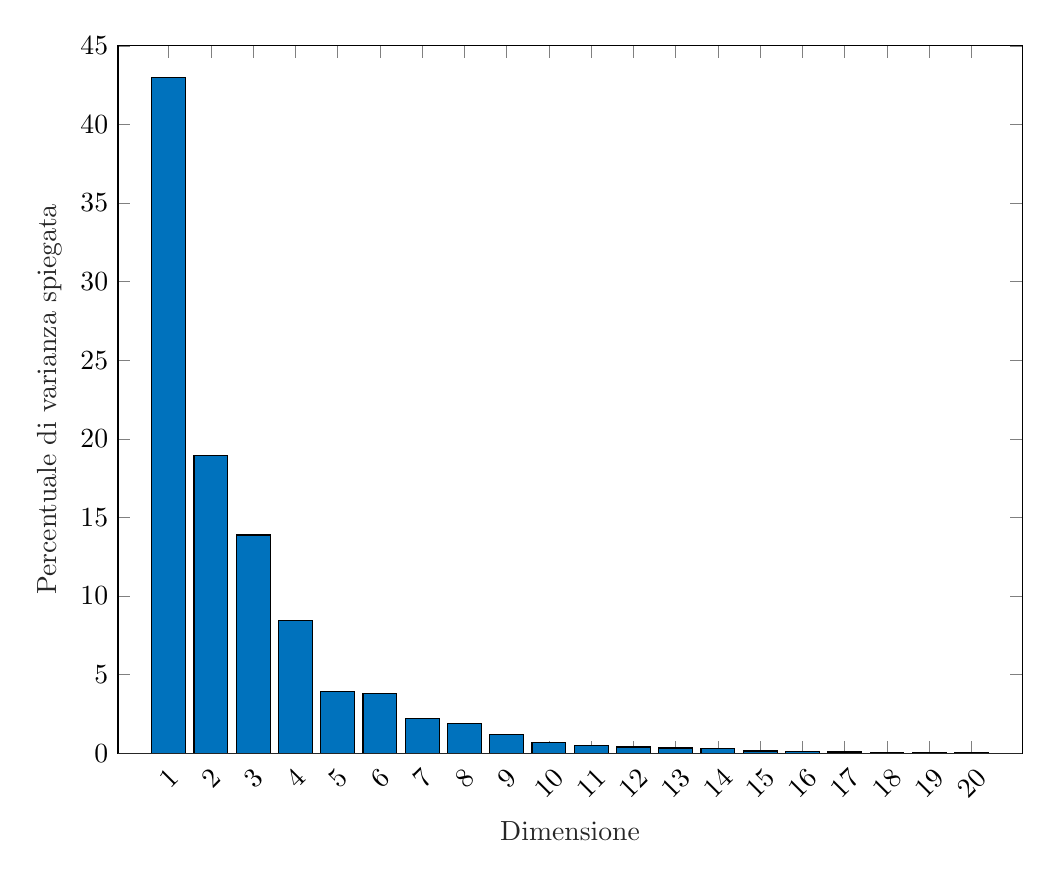
\begin{tikzpicture}

\begin{axis}[%
width=4.521in,
height=3.537in,
at={(0.758in,0.509in)},
scale only axis,
bar shift auto,
xmin=-0.2,
xmax=21.2,
xtick={ 1,  2,  3,  4,  5,  6,  7,  8,  9, 10, 11, 12, 13, 14, 15, 16, 17, 18, 19, 20},
xticklabel style={rotate=45},
xlabel style={font=\color{white!15!black}},
xlabel={Dimensione},
ymin=0,
ymax=45,
ylabel style={font=\color{white!15!black}},
ylabel={Percentuale di varianza spiegata},
axis background/.style={fill=white}
]
\addplot[ybar, bar width=0.8, fill=mycolor1, draw=black, area legend] table[row sep=crcr] {%
1	42.9768838681734\\
2	18.9438387765557\\
3	13.8822849835004\\
4	8.4482090947488\\
5	3.94157898572865\\
6	3.82236974172604\\
7	2.1924309730884\\
8	1.89045720135984\\
9	1.20660265153964\\
10	0.653960436042732\\
11	0.495294143310683\\
12	0.393730747866418\\
13	0.328488737865922\\
14	0.293967295915976\\
15	0.138279923173747\\
16	0.10776052667194\\
17	0.0785002474055965\\
18	0.0675765329298728\\
19	0.0457910948695177\\
20	0.0330722555146772\\
};
\addplot[forget plot, color=white!15!black] table[row sep=crcr] {%
-0.2	0\\
21.2	0\\
};
\end{axis}
\end{tikzpicture}%